% !TEX TS-program = pdflatex
% !TEX encoding = UTF-8 Unicode

% TO COMPILE: lmake (animal scrifices may be necessary)
%%%%%%%%%%%%%%%%%%%%%%%%%%%%%%%%%%%%%%%%%%%%%%%%%%%%%%%%%%%%%%%%%%%%%%%%%%
%																							                           %
%				                         PREAMBLE      							             %
%                                                                        %
%%%%%%%%%%%%%%%%%%%%%%%%%%%%%%%%%%%%%%%%%%%%%%%%%%%%%%%%%%%%%%%%%%%%%%%%%%
\documentclass[compress]{beamer}

\mode<presentation>
{
  \usetheme{Frankfurt}
  \usecolortheme{crane}
  \setbeamercovered{transparent}
}

% Package Setup
%%%%%%%%%%%%%%%%%%%%%%%%%%%%%%%%%%%%%%%%%%%%%%%%%%%%%%%%%%%%%%%%%%%%%%%%%%
%                                                                        %
%                                 PREAMBLE                               %
%                                                                        %
%%%%%%%%%%%%%%%%%%%%%%%%%%%%%%%%%%%%%%%%%%%%%%%%%%%%%%%%%%%%%%%%%%%%%%%%%%

%% PACKAGES
\usepackage[]{lineno}
\usepackage{fancyvrb}
%\linenumbers
\usepackage{amsmath}
\usepackage{microtype}
\usepackage{algorithmic}

%% GRAPHICS RELATED
\usepackage{graphicx}
\usepackage[outdir=./tmp/]{epstopdf}
\graphicspath{{../images/}{./}{./tmp/}}
\DeclareGraphicsExtensions{.eps, .pdf, .jpeg, .png}

%% CAPTION SETUP
\usepackage{float}
\usepackage[font=footnotesize]{caption}
\usepackage[font=small]{subcaption}
\captionsetup{belowskip=12pt,aboveskip=4pt}

%% BEAMER
\usepackage{multicol}
\usepackage{multirow}
\usepackage{array}				% Table Stuff
\usepackage{arydshln}
\usepackage{rotating}

%% BIBLIOGRAPHY
\bibliographystyle{ieeetr}

%% UNITS
\usepackage{siunitx}

%% EQUATIONS
%\numberwithin{equation}{section}

%%%%%%%%%%%%%%%%%%%%%%%%%%%%%%%%%%%%%%%%%%%%%%%%%%%%%%%%%%%%%%%%%%%%%%%%%%%
%                                                                         %
%                             Listing Setup                               %
%                                                                         %
%%%%%%%%%%%%%%%%%%%%%%%%%%%%%%%%%%%%%%%%%%%%%%%%%%%%%%%%%%%%%%%%%%%%%%%%%%%
\usepackage{listings}
\lstset{ %
    language=C++,
    basicstyle=\footnotesize\ttfamily,
    numbers=left,
    numberstyle=\tiny\color{gray},
    stepnumber=2,
    numbersep=5pt,
    backgroundcolor=\color{white},
    showspaces=false,
    showstringspaces=false,
    showtabs=false,
    frame=single,
    rulecolor=\color{black},
    tabsize=2,
    breaklines=true,
    breakatwhitespace=false,
    title=\lstname,
    keywordstyle=\color{blue},
    commentstyle=\color{OliveGreen},
    stringstyle=\color{orange}
}
\DeclareCaptionFont{white}{\color{white}}
\DeclareCaptionFormat{listing}{\colorbox[cmyk]{0.43, 0.35, 0.35, 0.01}{\parbox{\dimexpr\textwidth-2\fboxsep\relax}{#1#2#3}}}
\captionsetup[lstlisting]{format=listing,labelfont=white,textfont=white,singlelinecheck=false,margin=0pt,font={bf,footnotesize}}
%\lstnewenvironment{code}[1][]%
%{ \noindent\minipage{\linewidth}
%	\lstset{#1}
%}
%{\endminipage}
%% USER COMMANDS
\usepackage{isotope}
\newcommand{\iso}{\isotope}
\newcommand{\figurewidth}{\textwidth}
\newcommand{\micron}{$\mu$m}



% Preamble / Frst Size
%\setbeamersize{text margin left=5mm, text margin right 5mm}
\title[RPM8 Optimization] {Optimization of the RPM8 Detector with Genetic Algorithms}
\author[] {
    Matthew Urffer\inst{1}
}
\institute[University of Tennessee] { 
  \inst{1}%
  Department of Nuclear Engineering,
  University of Tennessee, Knoxville, TN
}

\date[] {March 3, 2013}
\pgfdeclareimage[height=0.5cm]{university-logo}{../images/utwordmarkhorz.png}
\logo{\pgfuseimage{university-logo}}

\begin{document}

\begin{frame}[plain]
  \titlepage
  \tiny
    \begin{center}
\centering{Financial support from the Domestic Nuclear Detection Office (DNDO) through Award No. 003387891 is gratefully acknowledged. 
  Any opinions, findings, and conclusions or recommendations expressed in this material are those of the presenter and do not necessarily reflect the views of DNDO.}
  \end{center}
\end{frame}

\begin{frame}{Table of Contents}
  \begin{multicols}{2}
    \tableofcontents
  \end{multicols}
\end{frame}


%%%%%%%%%%%%%%%%%%%%%%%%%%%%%%%%%%%%%%%%%%%%%%%%%%%%%%%%%%%%%%%%%%%%%%%%%%
%                                                                        %
%                          START OF CONTENT                              %
%                                                                        %
%%%%%%%%%%%%%%%%%%%%%%%%%%%%%%%%%%%%%%%%%%%%%%%%%%%%%%%%%%%%%%%%%%%%%%%%%%
\section{Introduction}
\subsection*{}
\begin{frame}{Introduction}
What geometry is best for the RPM8?
\begin{figure}
    \centering
    \begin{subfigure}[b]{0.25\textwidth}
        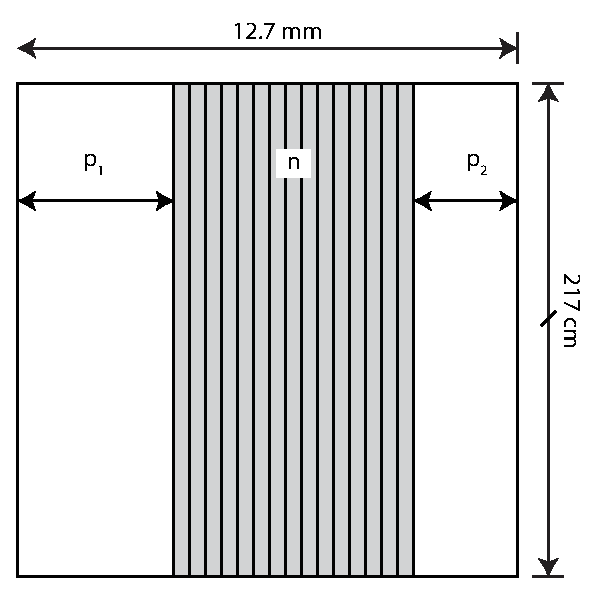
\includegraphics[width=\textwidth]{RPM8_Diagrams_OptDesign_A}
    \end{subfigure}
    ~
    \begin{subfigure}[b]{0.25\textwidth}
        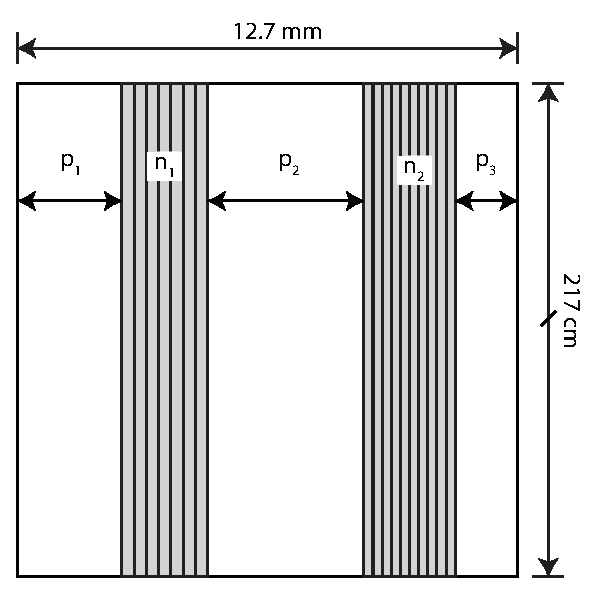
\includegraphics[width=\textwidth]{RPM8_Diagrams_OptDesign_B}
    \end{subfigure}

    \begin{subfigure}[b]{0.25\textwidth}
        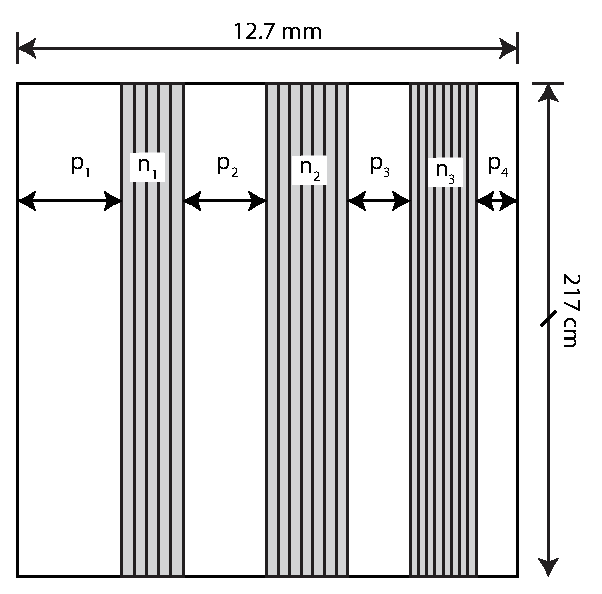
\includegraphics[width=\textwidth]{RPM8_Diagrams_OptDesign_C}
    \end{subfigure}
    ~
    \begin{subfigure}[b]{0.25\textwidth}
        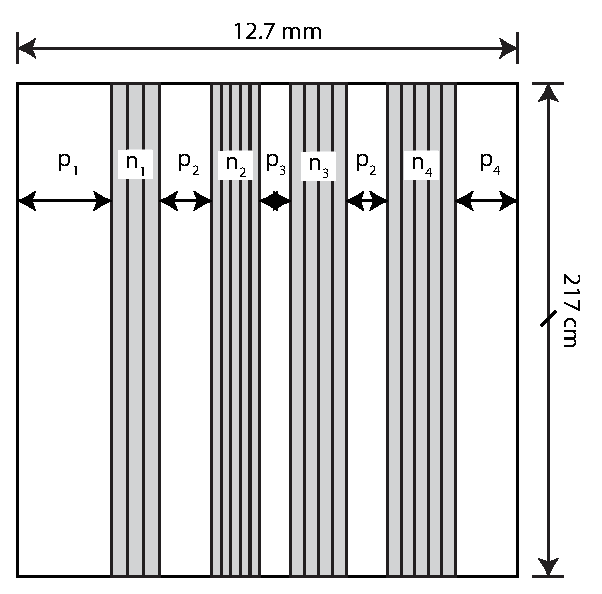
\includegraphics[width=\textwidth]{RPM8_Diagrams_OptDesign_D}
    \end{subfigure}
    \label{fig:OptDesignSchematics}
\end{figure}
Neturons will be moderated as they travel through the material, then wipped out by the absorber.
\end{frame}
%%%%%%%%%%%%%%%%%%%%%%%%%%%%%%%%%%%%%%%%%%%%%%%%%%%%%%%%%%%%%%%%%%%%%%%%%%
\begin{frame}{Design Constraints}
What do we mean by best?
\begin{itemize}
	\small
  \item Count rate? 
  \item Light output?
	\item Lowest cost / fabrication ease?
\end{itemize}
The design parameters were then:
\begin{itemize}
	\small
  \item The detector material
  \item The thickness of the detector material
  \item The spacing of detector layers
  \item The initial moderator thickness
\end{itemize}
\end{frame}
%%%%%%%%%%%%%%%%%%%%%%%%%%%%%%%%%%%%%%%%%%%%%%%%%%%%%%%%%%%%%%%%%%%%%%%%%%
\subsection{Previous Work}
\begin{frame}{Previous Work}
\begin{itemize}
	\small
	\item Have a working MCNPX model of the geometry
	\item Previous focused on a linear spacing of the films (simple)
	\item Have an idea on what thickness of moderator is necessary
		\begin{figure}
			\centering
			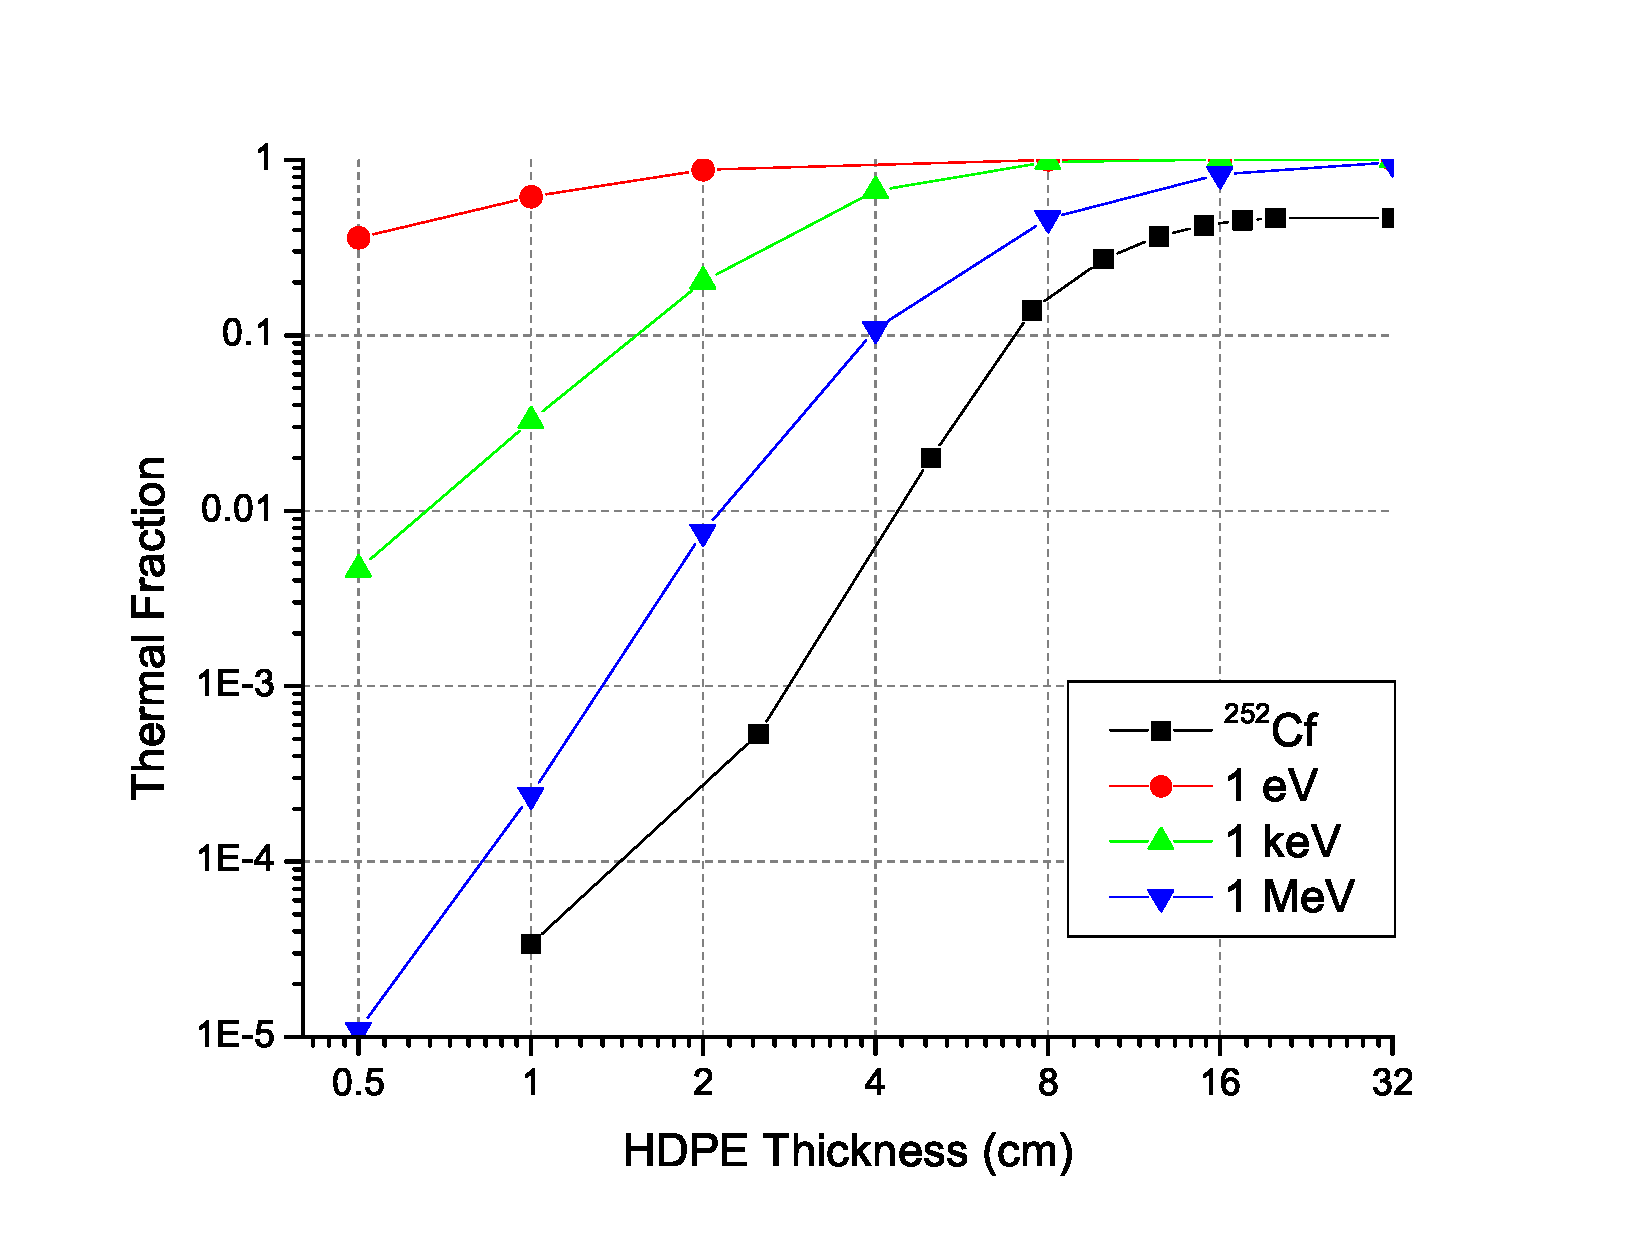
\includegraphics[width=0.75\textheight]{HDPEModThermalFraction}
		\end{figure}
	\item Don't know where the films go in the center
\end{itemize}
\centering
Optimization Problem!
\end{frame}
%%%%%%%%%%%%%%%%%%%%%%%%%%%%%%%%%%%%%%%%%%%%%%%%%%%%%%%%%%%%%%%%%%%%%%%%%%
%																							                           %
%% Genatic Algorthims introduction
%																							                           %
%%%%%%%%%%%%%%%%%%%%%%%%%%%%%%%%%%%%%%%%%%%%%%%%%%%%%%%%%%%%%%%%%%%%%%%%%%
\section{Genetic Algorithms}
\subsection{GA Introduction}
\begin{frame}{Genetic Algorithms}
A search technique mimicking natural evolution.
\begin{columns}[onlytextwidth]
  \begin{column}{0.45\textwidth}
    \small
    \begin{itemize}
      \item Population of candidate solutions is evolved toward better solutions
      \item Each candidate has properties that can be mutated and altered
      \item Traditionally solutions are represented as bit strings or trees
    \end{itemize}
    \end{column}
  \begin{column}{0.45\textwidth}
    \begin{figure}
		\tiny
		\begin{algorithmic}
      \WHILE{$error>goal$}
        \FORALL{$p \in P$}
          \STATE{Compute fitness}
        \ENDFOR
        \FORALL{$p \in P$}	
          \STATE{Choose individuals based on fitness}
          \STATE{Select individuals for next population}
          \STATE{Crossover selected individuals}
          \STATE{Mutate selected individual}
        \ENDFOR
      \ENDWHILE
    \end{algorithmic}
    \end{figure}
  \end{column}
\end{columns}
\end{frame}
\begin{frame}{Crossover Operations}
	\begin{columns}[onlytextwidth]
	\begin{column}{0.4\textwidth}
  \begin{itemize}
    \item Single point - choose a single point (two segments) to crossover
    \item Two point - choose two points (three segments) to crossover
    \item Uniform - Uniformly cross over based on some probability
  \end{itemize}
	\end{column}
	\begin{column}{0.55\textwidth}
    \begin{figure}
      \centering
      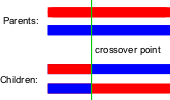
\includegraphics[width=0.3\textwidth]{SinglePointCrossover.png}
    \end{figure}
    \begin{figure}
      \centering
      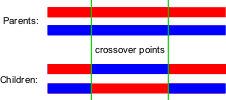
\includegraphics[width=0.3\textwidth]{TwoPointCrossover.png}
    \end{figure}
    \begin{figure}
      \centering
      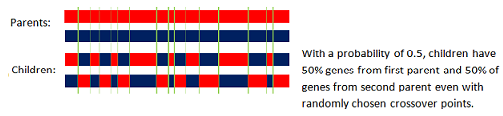
\includegraphics[width=\textwidth]{UniformCrossover.png}
    \end{figure}
	\end{column}
	\end{columns}
\end{frame}
\begin{frame}{Mutation Operations}
Mutations are designed to avoid local minima
\begin{columns}
\begin{column}{0.45\textwidth}
  \begin{itemize}
    \item Swap
    \item Flip - flips (inverts) all of the bits
  \end{itemize}
    \begin{figure}
      \centering
      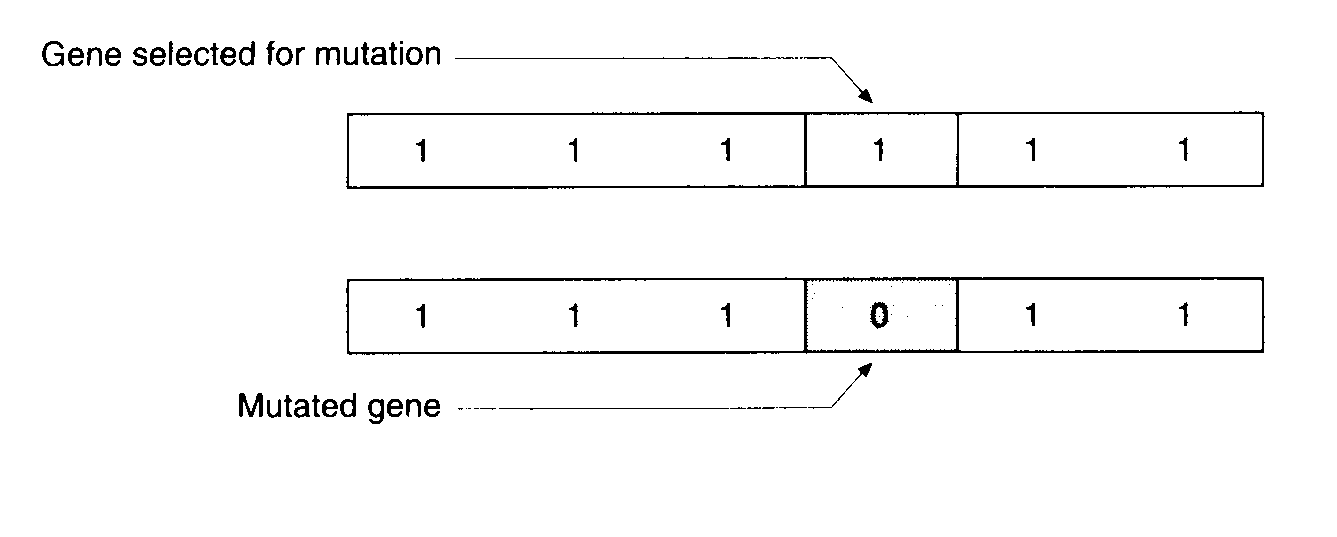
\includegraphics[width=0.4\textheight]{mutation_example.png}
    \end{figure}
	Typically set to be around a few percent
\end{column}
\begin{column}{0.45\textwidth}
\begin{figure}
	\centering
	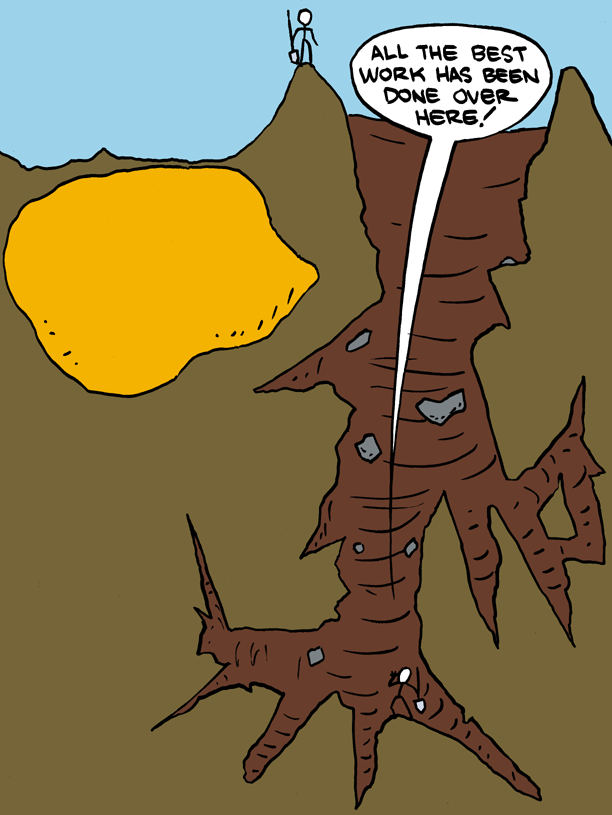
\includegraphics[width=0.75\textwidth]{AllTheBestWork.png}
\end{figure}
\end{column}
\end{columns}
\end{frame}
%%%%%%%%%%%%%%%%%%%%%%%%%%%%%%%%%%%%%%%%%%%%%%%%%%%%%%%%%%%%%%%%%%%%%%%%%%
\begin{frame}[fragile]{Choices, choices}
\centering
\tiny
\begin{Verbatim}[frame=single]
    ----------------------------------------------------------
                                                        F FN  
                                             F 5       F U  55
                                   F     F 5F  F     FFqBBMG05
                         F       FF1     N05 BBM F   F U8BBBMO
                      FF1       5 ZE     NN NBBB FF    1GMBB0 
                     F50Z5 F   1FMBBOF   F 5M20G  FF  5NBEOM 2
                    FFEBBB    5 M NM      5NBOO 8Bq   U8BBBBF5
                   1qZN MBZF F5OBME2F    F5Z8EB OZ   5 BBBBB 2
           5 F   F5MG M125   2BGMNF5     2MMM8MMF5   FBBBBBO 5
         UFF0 55  FEBMZGGF F  5BOGGN F   F5ZBNqB 5   1FBBZ GGG
    BNF5FGBN5BBNF FBBBBB 8E   5BMZO8q     2BBG 02     5BBB 1uq
    B 5q0BBBZqOq F1BBM5 51OZ 5 BB 5UE0     UBZN2     2ZBBBBEUU
    B OBBBBBG12 F 1BBO5 2F5   UEBBG2EBF   51BBBNU     JBBBBBG2
    BBBOG0BBB1 F  5 B qBB0 F 1uMB8B0FF   F2 BBBB F F U BB2 BBM
    B0MBB 0BB1F FFUUGBuNBM1 F ZB0j0OF   1 OBM 80    U8BBE5jNB8
    BUZBMZEFMNFF NMBBGFGB2  18BZ1UOB 5   OBq2UBEFF 1 BBq21 UBB
    BOG 5B 56BF 1BB0  UMB 5  BNUF FBM51 B8UFF5NBUF5FBB5UF 52MB
    BB 2 MZNZB 5 EqU 5 qM EFZGMq F5EBNZ  0 F 5 BMEZ BBB    2EB 
    ----------------------------------------------------------
    Symbolic Regression with Genetic Programing
    Matthew J. Urffer (matthew.urffer@gmail.com)
\end{Verbatim}
\end{frame}
%%%%%%%%%%%%%%%%%%%%%%%%%%%%%%%%%%%%%%%%%%%%%%%%%%%%%%%%%%%%%%%%%%%%%%%%%%
%                                                                        %
%                      Pyevole Introduction                              %
%                                                                        %
%%%%%%%%%%%%%%%%%%%%%%%%%%%%%%%%%%%%%%%%%%%%%%%%%%%%%%%%%%%%%%%%%%%%%%%%%%
\subsection{PyEvolve}
\begin{frame}{PyEvolve Introduction}
	\begin{itemize}
  \small
  \item PyEvolve is a genetic algorithm framework written in pure python
  \item Genetic Algorithm Features:
    \begin{itemize}
      \item Crossover operations (single point, two point, uniform)
      \item Mutator operations (swap, flip)
      \item Selection operations (rank, uniform, tournament, roulette)
    \end{itemize}
  \item Additional Features:
    \begin{itemize}
      \item Run statistics
      \item Convergence criteria
      \item Function callbacks
    \end{itemize}
  \end{itemize}
  \begin{figure}
    
\includegraphics[width=0.2\textwidth]{PyEvolveLogo.png}
  \end{figure}
\end{frame}
\begin{frame}{PyEvolve - Belly of the Lizard}
	Representation of the the Genetic Algorithm
  \begin{itemize}
    \item \texttt{GSimpleGA} genetic algorithm
    \item \texttt{GPopulation} - the population
    \item \texttt{Initializators} - initialization methods
    \item \texttt{Mutators} - collection of mutator methods
    \item \texttt{Crossovers} - collection of crossover methods
    \item \texttt{Selectors} - collection of selection methods
  \end{itemize}
  Representation of an individual
  \begin{itemize}
    \item Bit string representation \texttt{10010101}
    \item Defined in \texttt{G1DBinaryString.py}
		\item Other representations are available (tree, 2D list)
  \end{itemize}
\end{frame}
%%%%%%%%%%%%%%%%%%%%%%%%%%%%%%%%%%%%%%%%%%%%%%%%%%%%%%%%%%%%%%%%%%%%%%%%%%
%																							                           %
%								             Methods 					                           %
%																							                           %
%%%%%%%%%%%%%%%%%%%%%%%%%%%%%%%%%%%%%%%%%%%%%%%%%%%%%%%%%%%%%%%%%%%%%%%%%%
\section{Methods}
%%%%%%%%%%%%%%%%%%%%%%%%%%%%%%%%%%%%%%%%%%%%%%%%%%%%%%%%%%%%%%%%%%%%%%%%%%
\begin{frame}{Optimization Formulation}
The optimization of the films was formulated as finding the minimum mass of \iso[6]{Li} for a given detector material necessary to fulfill an interaction rate of \SI{2.5}{cps\per\nano\gram\iso[252]{Cf}} while maintaining a intrinsic gamma rejection ratio of \num{1.e-6}.
\end{frame}
%%%%%%%%%%%%%%%%%%%%%%%%%%%%%%%%%%%%%%%%%%%%%%%%%%%%%%%%%%%%%%%%%%%%%%%%%%
\subsection{Geometry Description}
\begin{frame}[fragile]{Gigantic Genome Geometries}
Genome BitString Representation
\begin{itemize}
  \item Divide the RPM8 width into even slices
  \item Compact representation of geometry, suitable for GA
  \item \verb+1+ - represents a detector assembly slice
  \item \verb+0+ - represents a moderator slice
  \item Example: \verb+001000+
  \begin{itemize}
    \item Each slice is \SI{2.12}{\centi\meter}
    \item Two slices of moderator, followed by one assembly slice followed by three additional slices of moderator
  \end{itemize}
\end{itemize}
\end{frame}
%%%%%%%%%%%%%%%%%%%%%%%%%%%%%%%%%%%%%%%%%%%%%%%%%%%%%%%%%%%%%%%%%%%%%%%%%%
\begin{frame}[fragile]{Computional Size}
\small
\begin{itemize}
  \item Each bit has two options, \verb+0+ or \verb+1+
  \item $2^n$ combinations for the search space - NP Hard!
  \item Each run takes about 1.72 minutes (16 cores)
\end{itemize}
\begin{table}
    \caption[Genome Bit String Geometries]{Bit String Simplified Geometetry Descriptions}
    \label{tab:BitStringGeo}
    \centering
    \tiny
    \begin{tabular}{ m{1.5cm} | m{1.5cm} m{1.5cm} m{1.5cm}  m{1.5cm}}
      Genome Length&Films Per Assembly&Slice Thickness&Light Guide Thickness&Possible Geomeries \\
      \hline
      \hline
      3&4&4.23&1.058&7 \\
      4&4&3.18&0.794&15 \\
      5&3&2.54&0.847&31 \\
      6&3&2.12&0.706&63 \\
      7&3&1.81&0.605&127 \\ 
      10&3&1.27&0.423&1023 \\
      13&2&0.98&0.488&8191 \\
      26&1&0.49&0.488&67108863 \\
    \end{tabular}
\end{table}
\end{frame}
%%%%%%%%%%%%%%%%%%%%%%%%%%%%%%%%%%%%%%%%%%%%%%%%%%%%%%%%%%%%%%%%%%%%%%%%%%
\begin{frame}
\begin{figure}
    \centering
    \begin{subfigure}[b]{0.45\textwidth}
        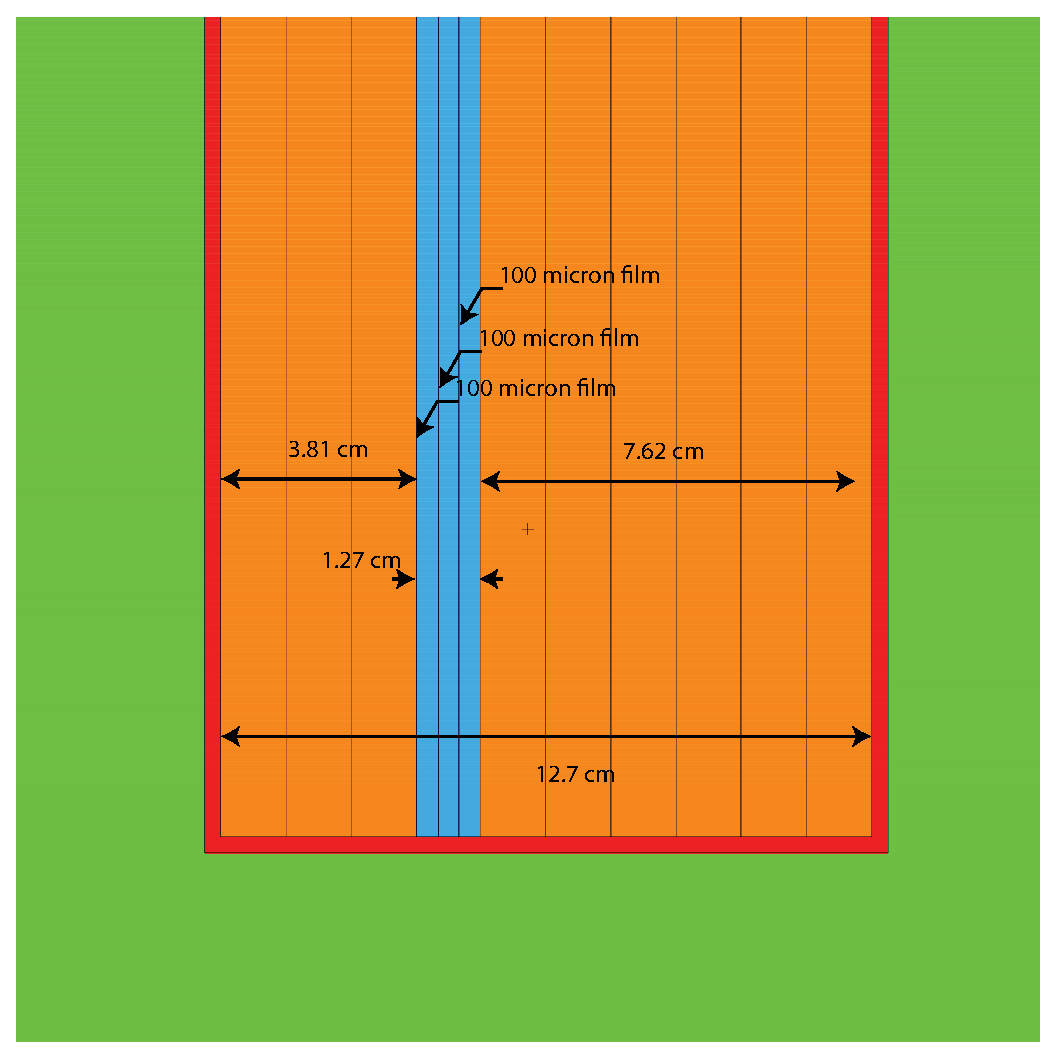
\includegraphics[width=\textwidth]{RPM8_Diagrams_MCNPXRender_10Opt}
    \end{subfigure}%
    ~
    \begin{subfigure}[b]{0.45\textwidth}
        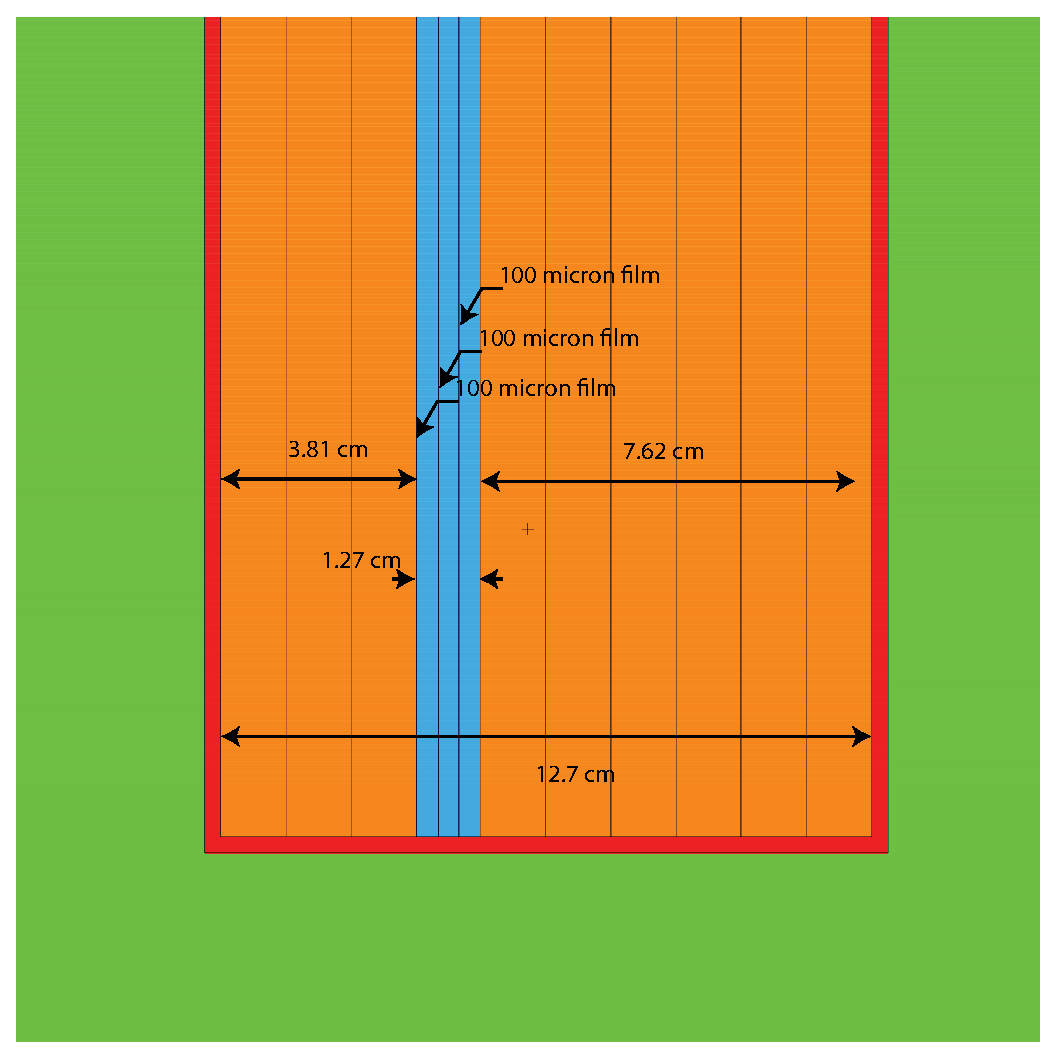
\includegraphics[width=\textwidth]{RPM8_Diagrams_MCNPXRender_26Opt}
    \end{subfigure}
    \caption{MCNPX rendering of layered geometry}
    \label{fig:MCNPXRendering}
\end{figure}
\end{frame}
%%%%%%%%%%%%%%%%%%%%%%%%%%%%%%%%%%%%%%%%%%%%%%%%%%%%%%%%%%%%%%%%%%%%%%%%%%
\subsection{Implemented Genetic Operators}
%%%%%%%%%%%%%%%%%%%%%%%%%%%%%%%%%%%%%%%%%%%%%%%%%%%%%%%%%%%%%%%%%%%%%%%%%%
\begin{frame}[fragile]{Mutation, Crossover and Selection}
  Operators from the PyEvolve toolkit
  \begin{itemize}
    \item Mutation - Flip Operator (2\%)
    \item Crossover - Single Point (90\%)
    \item Selection - Tournament Selection
  \end{itemize}
\end{frame}
%%%%%%%%%%%%%%%%%%%%%%%%%%%%%%%%%%%%%%%%%%%%%%%%%%%%%%%%%%%%%%%%%%%%%%%%%%
\begin{frame}{Fitness Function}
The fitness function was choosen to count rate per mass of \iso[6]{Li}, provided that the geometry meet the total count rate criteria.
If it failed to meet the count rate criteria a zero fitness was returned \eqref{eqn:FitnessFun}.
	\tiny
	\begin{align}
			\label{eqn:FitnessFun}
			f(\vec{x})
			= \begin{cases}
			0 & \text{if}~\text{countRate}(\vec{x}) \leq \SI{2.5}{cps\per\nano\gram\iso[252]{Cf}} \\
			\text{countRatePerMass}(\vec{x}) & \text{otherwise}
			\end{cases}
	\end{align}
\begin{columns}[onlytextwidth]
  \begin{column}{0.5\textwidth}
\small
	Computationally intensive to calculate the fitness function 
	\begin{itemize}
		\item Memoization with dictionaries
		\item Multithreading for items not in the dictionary
		\tiny
		\begin{itemize}
			\item This made it sensitive while running
			\item Future work would be to use the PyEvovle multithreading option
		\end{itemize}
	\end{itemize}
	\end{column}
	\begin{column}{0.4\textwidth}
    \begin{figure}
      \centering
      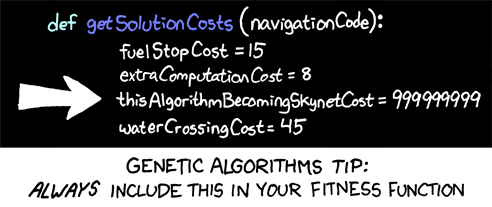
\includegraphics[width=\textwidth]{genetic_algorithms}
    \end{figure}
	\end{column}
\end{columns}
\end{frame}
%%%%%%%%%%%%%%%%%%%%%%%%%%%%%%%%%%%%%%%%%%%%%%%%%%%%%%%%%%%%%%%%%%%%%%%%%%
%																							                           %
%													Results 						                           %
%																							                           %
%%%%%%%%%%%%%%%%%%%%%%%%%%%%%%%%%%%%%%%%%%%%%%%%%%%%%%%%%%%%%%%%%%%%%%%%%%
\section{Results}
\subsection{Validation}
\begin{frame}{Validation}
Validation of optimal solution can be observed directly for low dimensional searches
\begin{table}
    \caption[3 Bit Genome Results]{Bit String Simplified Geometry Descriptions}
    \label{tab:BitStringGeo}
    \centering
    \tiny
    \begin{tabular}{ p{1.5cm} | p{1.5cm} p{1.5cm}  p{1.5cm}}
			Genome&Mass Li-6&Count Rate& Count Rate per Mass \\
      \hline
      \hline
			010&16.7&2.9&0.175 \\ 
			\hline
			011&33.5&3.3&0.100 \\
			001&16.7&1.28&0.074 \\
			111&50.3&4.6&0.091 \\
			110&33.5&4.2&0.125 \\ 
			100&16.7&2.5&0.147 \\
			101&33.5&3.9&0.116 \\
      \hline
    \end{tabular}
\end{table}
Similarly for other low dimensional search spaces
\end{frame}

\begin{frame}[fragile]{Bootstrapped Genomes and Engineering Judgment}
\begin{itemize}
	\item Observed that all optimal solutions in low dimensions have moderator and reflector
	\item Possibility to reduce search space by setting moderator and reflector bits
	\item Possibility to initialize solutions for higher dimensions from lower ones
	\begin{itemize}
		\item Example: \verb+010+ $\to$ \verb+01000+ $\to$ \verb+0010000100000+
		\item Danger is not having enough diversity to avoid local minima
	\end{itemize}
\end{itemize}
\end{frame}

\begin{frame}[fragile]{Optimal Geometries}
\begin{table}
    %\caption[Optimal Bit String Geometries]{Genatic Algothrim Optimal Geometries}
    \centering
    \tiny
    \begin{tabular}{ p{0.75cm} | p{1cm} p{3.25cm} p{0.75cm} p{1cm} p{1cm}}
      Genome Length&Films Per Assembly&Optimal Geometry&Mass \iso[6]{Li}(g)&CPS per ng \iso[252]{Cf} & Count Rate per Mass \iso[6]{Li} (cps/g) \\
      \hline
      \hline
      3&4&\verb+010+&16.75&2.93&0.175 \\
      4&4&\verb+0100+& & & \\
      5&3&\verb+01000+&12.56&2.89&0.230 \\
      6&3&\verb+010000+&12.56&2.88&0.230 \\
      7&3&\verb+0100000+&12.56&2.84&0.226 \\ 
      10&3&\verb+0100000000+&12.56&2.68&0.214 \\
      10&3&\verb+0010000000+&12.56&2.93&0.233 \\
      10&3&\verb+0001000000+&12.56&2.95&0.235 \\
      13&2&\verb+00010010000000+&16.75&3.88&0.232 \\
      13&2&\verb+00100010000000+&16.75&3.90&0.233 \\
      13&2&\verb+00100100000000+&16.75&3.87&0.231 \\
      26&1&\verb+00000110110000000010000000+&20.94&4.33&0.206 \\
      26&1&\verb+00001010001000100000000000+&16.75&4.20&0.251 \\
    \end{tabular}
\end{table}
\end{frame}
%%%%%%%%%%%%%%%%%%%%%%%%%%%%%%%%%%%%%%%%%%%%%%%%%%%%%%%%%%%%%%%%%%%%%%%%%%
\begin{frame}{Optimal Geometries Rendered}
\begin{figure}
    \centering
    \begin{subfigure}[b]{0.45\textwidth}
        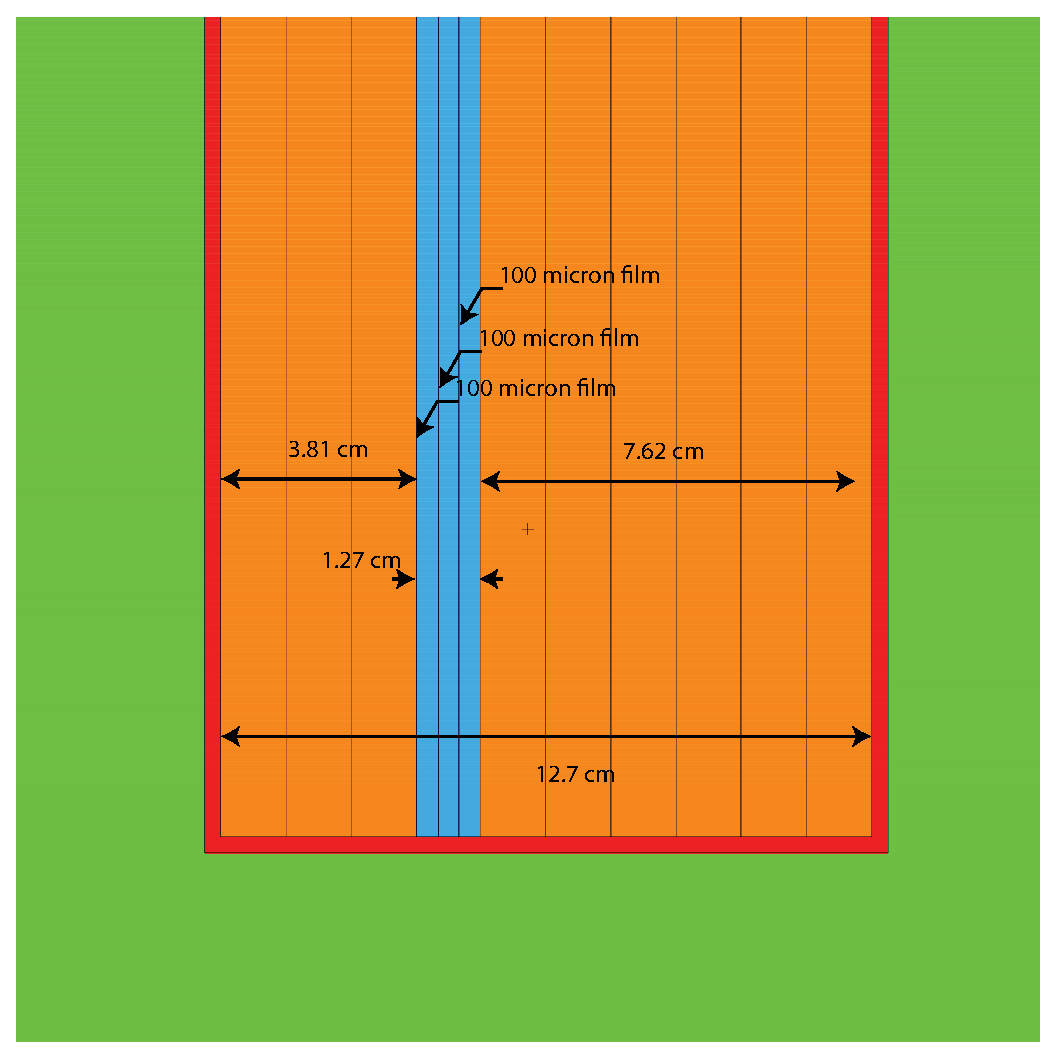
\includegraphics[width=\textwidth]{RPM8_Diagrams_MCNPXRender_10Opt}
    \end{subfigure}%
    ~
    \begin{subfigure}[b]{0.45\textwidth}
        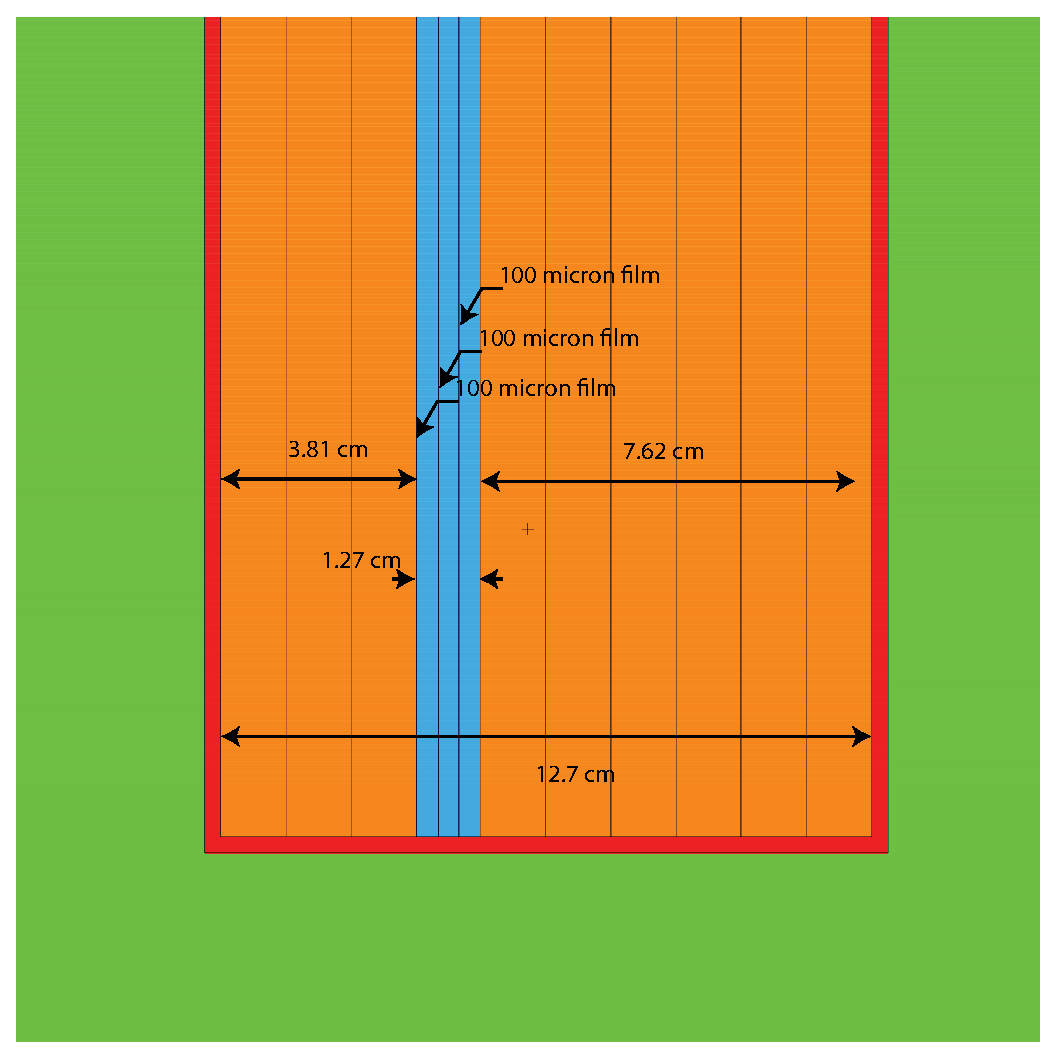
\includegraphics[width=\textwidth]{RPM8_Diagrams_MCNPXRender_26Opt}
    \end{subfigure}
    \caption{MCNPX rendering of layered geometry}
    \label{fig:MCNPXRendering}
\end{figure}
\end{frame}
%%%%%%%%%%%%%%%%%%%%%%%%%%%%%%%%%%%%%%%%%%%%%%%%%%%%%%%%%%%%%%%%%%%%%%%%%%
\subsection{Timing and Run Information}
\begin{frame}{Number of Geometries and Search Space}
Benefit of GA becomes apparent at higher search spaces!
\begin{table}
    %\caption[Optimal Bit String Geometries]{Genatic Algothrim Optimal Geometries}
    \centering
    \tiny
    \begin{tabular}{ p{0.75cm} | p{1cm} p{1cm} p{1cm} p{1cm} p{1cm}}
      Genome Length&Population Size&Number Runs&Average Generations&Fraction of Search Space Covered&Average Geometries Simulated \\
      \hline
      \hline
      3&6&20&4.6&100\%&24.5 \\
			4&8&18&3.8&100\%&30.7 \\
			5&10&18&6.0&100\%& 60.0 \\
			6&12&19&7.6&100\%&91.6 \\
			7&14&16&8.8&0.87\%&122.7 \\
			10&20&12&26.8&0.47\%& 536.7 \\
			13&26&8&19.0&0.18\% &494.0\\
			26&52&2&8.5&0.0014\% &442.0\\
    \end{tabular}
\end{table}
\end{frame}

\section{Conclusions}
%%%%%%%%%%%%%%%%%%%%%%%%%%%%%%%%%%%%%%%%%%%%%%%%%%%%%%%%%%%%%%%%%%%%%%%%%%
%																							                           %
%												Conclusions						                           %
%																							                           %
%%%%%%%%%%%%%%%%%%%%%%%%%%%%%%%%%%%%%%%%%%%%%%%%%%%%%%%%%%%%%%%%%%%%%%%%%%
\begin{frame}{Summary}
Cost trade offs
\begin{itemize}
	\item Assumed \iso[6]{Li} was the most expensive part
	\item Fabrication cost for a complicated design might hinder this
	\item Is the space thick enough to get the light out?
\end{itemize}
Can significantly reduce the amount of \iso[6]{Li} needed
\end{frame}
\begin{frame}{Future Work}
\begin{itemize}
	\item Improve performance on GA
	\small
	\begin{itemize}
		\item Can play with mutation rate and crossover rate
		\item Can play with population size and selection
		\item Use PyEvolve multiprocessing instead of mine - might remove code sensitivity
	\end{itemize}
	\normalsize
	\item Use a 1D transport code
	\item Run for different materials
	\item More runs at higher lengths
\end{itemize}
\end{frame}
\begin{frame}
	\centering
\begin{figure}
  
\includegraphics[height=6cm]{Questions.eps}
\end{figure}
\end{frame}
%%%%%%%%%%%%%%%%%%%%%%%%%%%%%%%%%%%%%%%%%%%%%%%%%%%%%%%%%%%%%%%%%%%%%%%%%%%
% BILBIOLGRAPHY
%\begin{frame}[plain,allowframebreaks]
%\frametitle{Works Cited}
%	\tiny
%  \bibliography{../Zotero}
%\end{frame}

%%%%%%%%%%%%%%%%%%%%%%%%%%%%%%%%%%%%%%%%%%%%%%%%%%%%%%%%%%%%%%%%%%%%%%%%%%%
% APPENDIX
%%%%%%%%%%%%%%%%%%%%%%%%%%%%%%%%%%%%%%%%%%%%%%%%%%%%%%%%%%%%%%%%%%%%%%%%%%%
\begin{frame}{Geometry for HDPE Moderation}
\begin{figure}
  \begin{subfigure}[b]{0.45\textwidth}
    \centering
    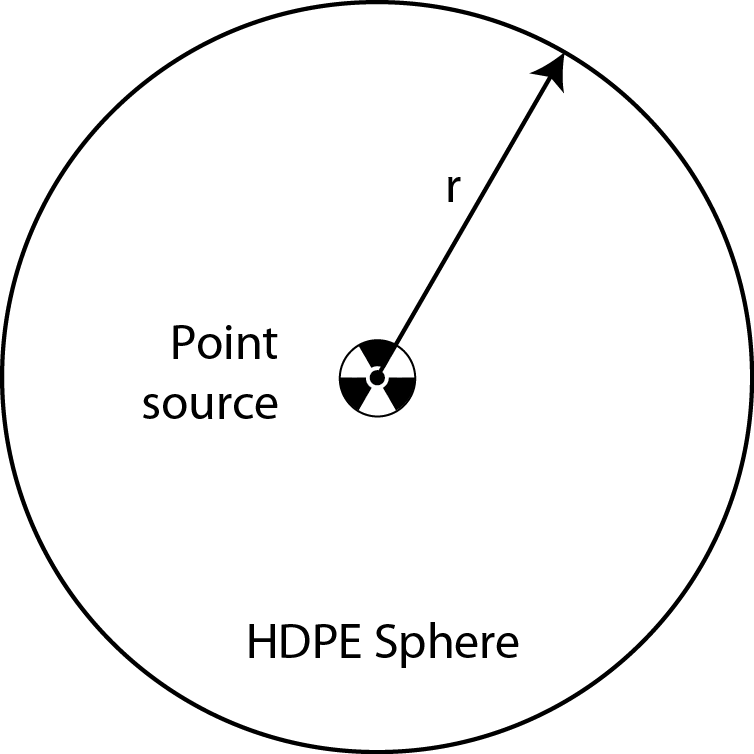
\includegraphics[width=\textwidth]{HDPEModeration_PointSrcGeo}
    \caption{Geometry of mono energetic point source}
  \end{subfigure}%
  ~
  \begin{subfigure}[b]{0.45\textwidth}
    \centering
    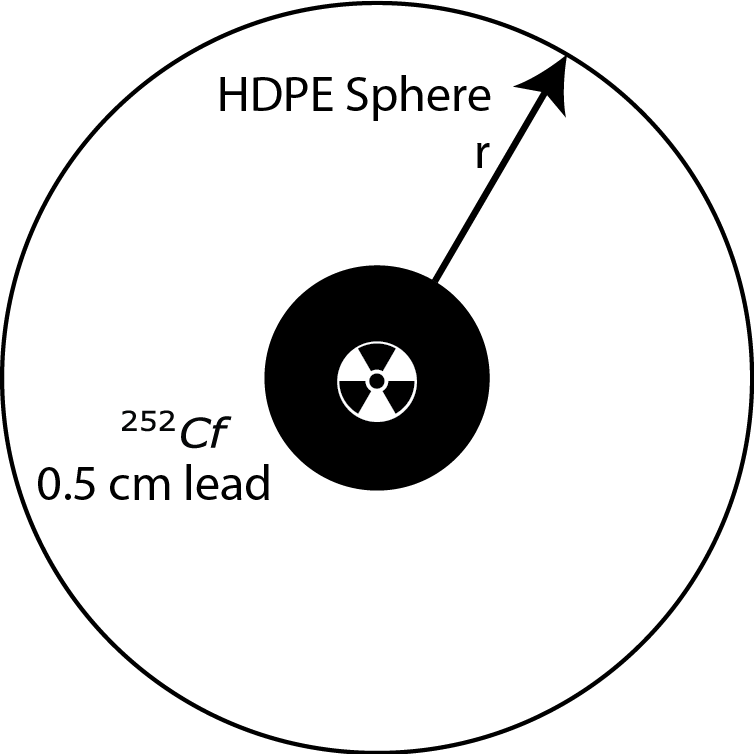
\includegraphics[width=\textwidth]{HDPEModeration_Cf252SrcGeo}
    \caption{Geometry of \isotope[252]{Cf} source}
  \end{subfigure}
  \caption{Simulated Geometry}
\end{figure}
\end{frame}
%%%%%%%%%%%%%%%%%%%%%%%%%%%%%%%%%%%%%%%%%%%%%%%%%%%%%%%%%%%%%%%%%%%%%%%%%%%

\end{document}


